\documentclass{article}
%\usepackage{harvard}
\usepackage[english]{babel}

% Set page size and margins
\usepackage[a4paper,top=2cm,bottom=2cm,left=3cm,right=3cm,marginparwidth=1.75cm]{geometry}

% Useful packages
\usepackage{amsmath}
\usepackage{graphicx}
\usepackage[colorlinks=true, allcolors=blue]{hyperref}
\usepackage{amsfonts} 


\title{Neural architecture search with target hardware control}
\author{Firsov Sergey\\
        Intelligent Systems Phystech}

\begin{document}
\maketitle

\begin{abstract}
The paper examines the problem of deep learning model selection with respect to target hardware. We propose a method for neural architecture search (NAS) that accounts for hardware constraints and model complexity. The complexity of the model is measured by the number of parameters, while the hardware constraints are represented by the overall latency of network operations on the target device. 

This approach builds upon Differentiable Architecture Search (DARTS), treating network structural parameters as functions of a complexity parameter, and extends it by incorporating latency-aware optimization inspired by FBNet. By introducing Gumbel-Softmax sampling and hypernetworks, we enable simultaneous optimization of multiple architectures across a range of complexity levels. This results in a single optimization process that identifies a family of architectures tailored to different computational budgets, reducing search time and resources.
\end{abstract}

\section{Introduction}

Selecting an appropriate architecture for deep learning models is a crucial task that directly impacts model efficiency and performance. With deep learning continuing to push computational limits, researchers face the challenge of finding a balance between model complexity, accuracy, and resource consumption. Recent advances in Neural Architecture Search (NAS)~\cite{nas} techniques, such as Differentiable Architecture Search (DARTS)~\cite{liu2019darts}, seek to automate this process by exploring large search spaces of possible network structures. However, these methods often struggle with high computational requirements and the need for architecture adjustments when model complexity or target hardware changes~\cite{yakovlev2021neural}. % ~\cite{Wu_2019_CVPR},

One of the significant developments in NAS is the introduction of hardware-aware models. For example, FBNet~\cite{Wu_2019_CVPR} incorporates latency into the architecture search process, optimizing not only model performance but also hardware efficiency. This approach addresses the mismatch between FLOPs and actual hardware performance, a limitation of many prior NAS methods. FBNet achieves this through gradient-based optimization and Gumbel-Softmax sampling, which dramatically reduce the search costs while generating a family of hardware-optimized models.
% MnasNet

Similar ideas are used in ProxylessNAS~\cite{proxylessnas}, which solves the problem of high memory and computing costs by optimizing architectures directly on large tasks and target hardware platforms, without using proxy tasks. ProxylessNAS introduces a direct search engine (Reinforce sampling) for learning architectures on large datasets and simulates operation delays to account for hardware limitations. However, this approach requires careful calibration, as enhanced learning often suffers from high variance.

Building on these ideas, our work improves upon DARTS-CC~\cite{yakovlev2021neural} %тут как будто переделать надо
, a NAS approach that uses hypernetworks to control model complexity during architecture search. Unlike other methods that search for individual architectures at different complexity levels, DARTS-CC generates multiple architectures in a single optimization process. Inspired by FBNet, we extend DARTS-CC by integrating latency-aware optimization and replacing the scalar complexity parameter with a simplex-based representation of architecture choices. This enables simultaneous search for architectures optimized across multiple complexity and latency levels, further reducing NAS time, and ensuring deployability across diverse hardware environments.

Our contributions can be summarized as follows:
\begin{itemize}
    \item We extend DARTS-CC by incorporating hardware latency into the optimization process. This enables the discovery of architectures that are not only accurate, but also efficient on target devices.
    \item We replace the scalar complexity parameter in DARTS-CC with a simplex-based representation, allowing the use of Gumbel-Softmax sampling for flexible architecture optimization.
    \item We propose a unified framework that combines latency-aware optimization, hypernetworks, and Gumbel-Softmax sampling to generate a family of architectures in a single optimization run.
    \item We validate our method on multiple datasets and hardware platforms, demonstrating improved efficiency and flexibility compared to existing NAS approaches.
\end{itemize}

%%%%%%%%%%%%%%%%%%%%%%%%%%
\subsection{Proposed Method}
The proposed method formulates Neural Architecture Search (NAS) as an optimization problem that simultaneously considers model accuracy, complexity, and hardware efficiency.

\textbf{Problem Formulation.} In conventional DARTS the goal is to find architectural parameters \(\boldsymbol{\alpha} \in \mathcal{A}\) and model weights \(\boldsymbol{w} \in \mathcal{W}\) such that the loss function \(L(\boldsymbol{w}, \boldsymbol{\alpha})\) is minimized. The optimization problem can be formulated as follows:

\[
\min_{\boldsymbol{\alpha} \in \mathcal{A}} \big[L(\boldsymbol{w}^*(\boldsymbol{\alpha}), \boldsymbol{\alpha}) \big],
\]

subject to:
\[
\boldsymbol{w}^*(\boldsymbol{\alpha}) = \arg \min_{\boldsymbol{w} \in \mathcal{W}} L(\boldsymbol{w}, \boldsymbol{\alpha}),
\]
where \(L(\boldsymbol{w}, \boldsymbol{\alpha})\) represents the task loss.  \\
However, DARTS does not account for flexibility in controlling model complexity or hardware constraints. So we propose these extensions to the DARTS framework to address its limitations:

\textbf{First Step. Architecture Representation.} The architectural parameters \(\boldsymbol{\alpha}\) we define as a function of a complexity parameter \(\lambda \in \mathbb{R}^+\)~\cite{yakovlev2021neural}, which maps to the architecture space \(\mathcal{A}\):
\[
\boldsymbol{\alpha}: \lambda \to \mathcal{A}.
\]
This allows generates multiple architectures with different complexity in a single optimization process.

\textbf{Second Step. Simplex-Based Complexity Control.} Instead of using a scalar parameter \(\lambda\), we introduce a simplex-based representation \( \boldsymbol{S} \in \Delta^{k-1}\), where \(\Delta^{k-1}\) denotes a \((k-1)\)-dimensional simplex,  \(k\) - is number of operations. The parameter \(\boldsymbol{S}\) is sampled using the Gumbel-Softmax distribution to allow differentiable selection of architectural components:
\[
\boldsymbol{S} \sim \text{GumbelSoftmax}(\boldsymbol{\theta}).
\]

\textbf{Third Step. Latency regularization.} To account for hardware constraints, we introduce a latency lookup table that records the latency of each operation on the target device. The total latency is computed as a weighted sum of the latencies of the operations selected by the architecture.

The objective function now becomes:
\[
\mathbb{E}_{\boldsymbol{S} \sim \text{GumbelSoftmax}} \big[L(\boldsymbol{w}^*(\boldsymbol{S}), \boldsymbol{\alpha}(\boldsymbol{S})) + \lambda \cdot \text{Reg}(\boldsymbol{\alpha}(\boldsymbol{S})) + \kappa \cdot \text{Latency}(\boldsymbol{\alpha}(\boldsymbol{S}))\big].
\]

So by using complexity dependence architecture parameters we generate multiple architectures in a single optimization process, by replacing the scalar complexity parameter with the simplex representation, we achieve finer control over architectural complexity, enabling flexible optimization across a range of hardware and resource constraints and by using latency lookup table, we can control hardware constraints.  \\

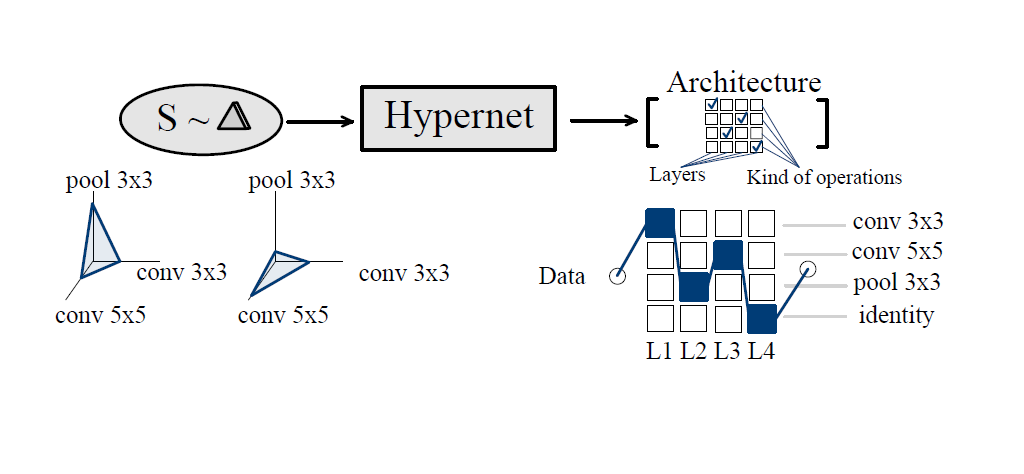
\includegraphics[width=1\linewidth]{picture.png}
%Еще нужна картирнка

\bibliographystyle{plain}
\bibliography{sample}

\end{document}